%==========================================================
% O título fica na página deitada, junto do mapa, para não ficar sozinho no fim da página anterior.
\begin{landscape}
\section{\textit{Story map}}\label{sec:storymap}

\begin{figure}[H]
\centering
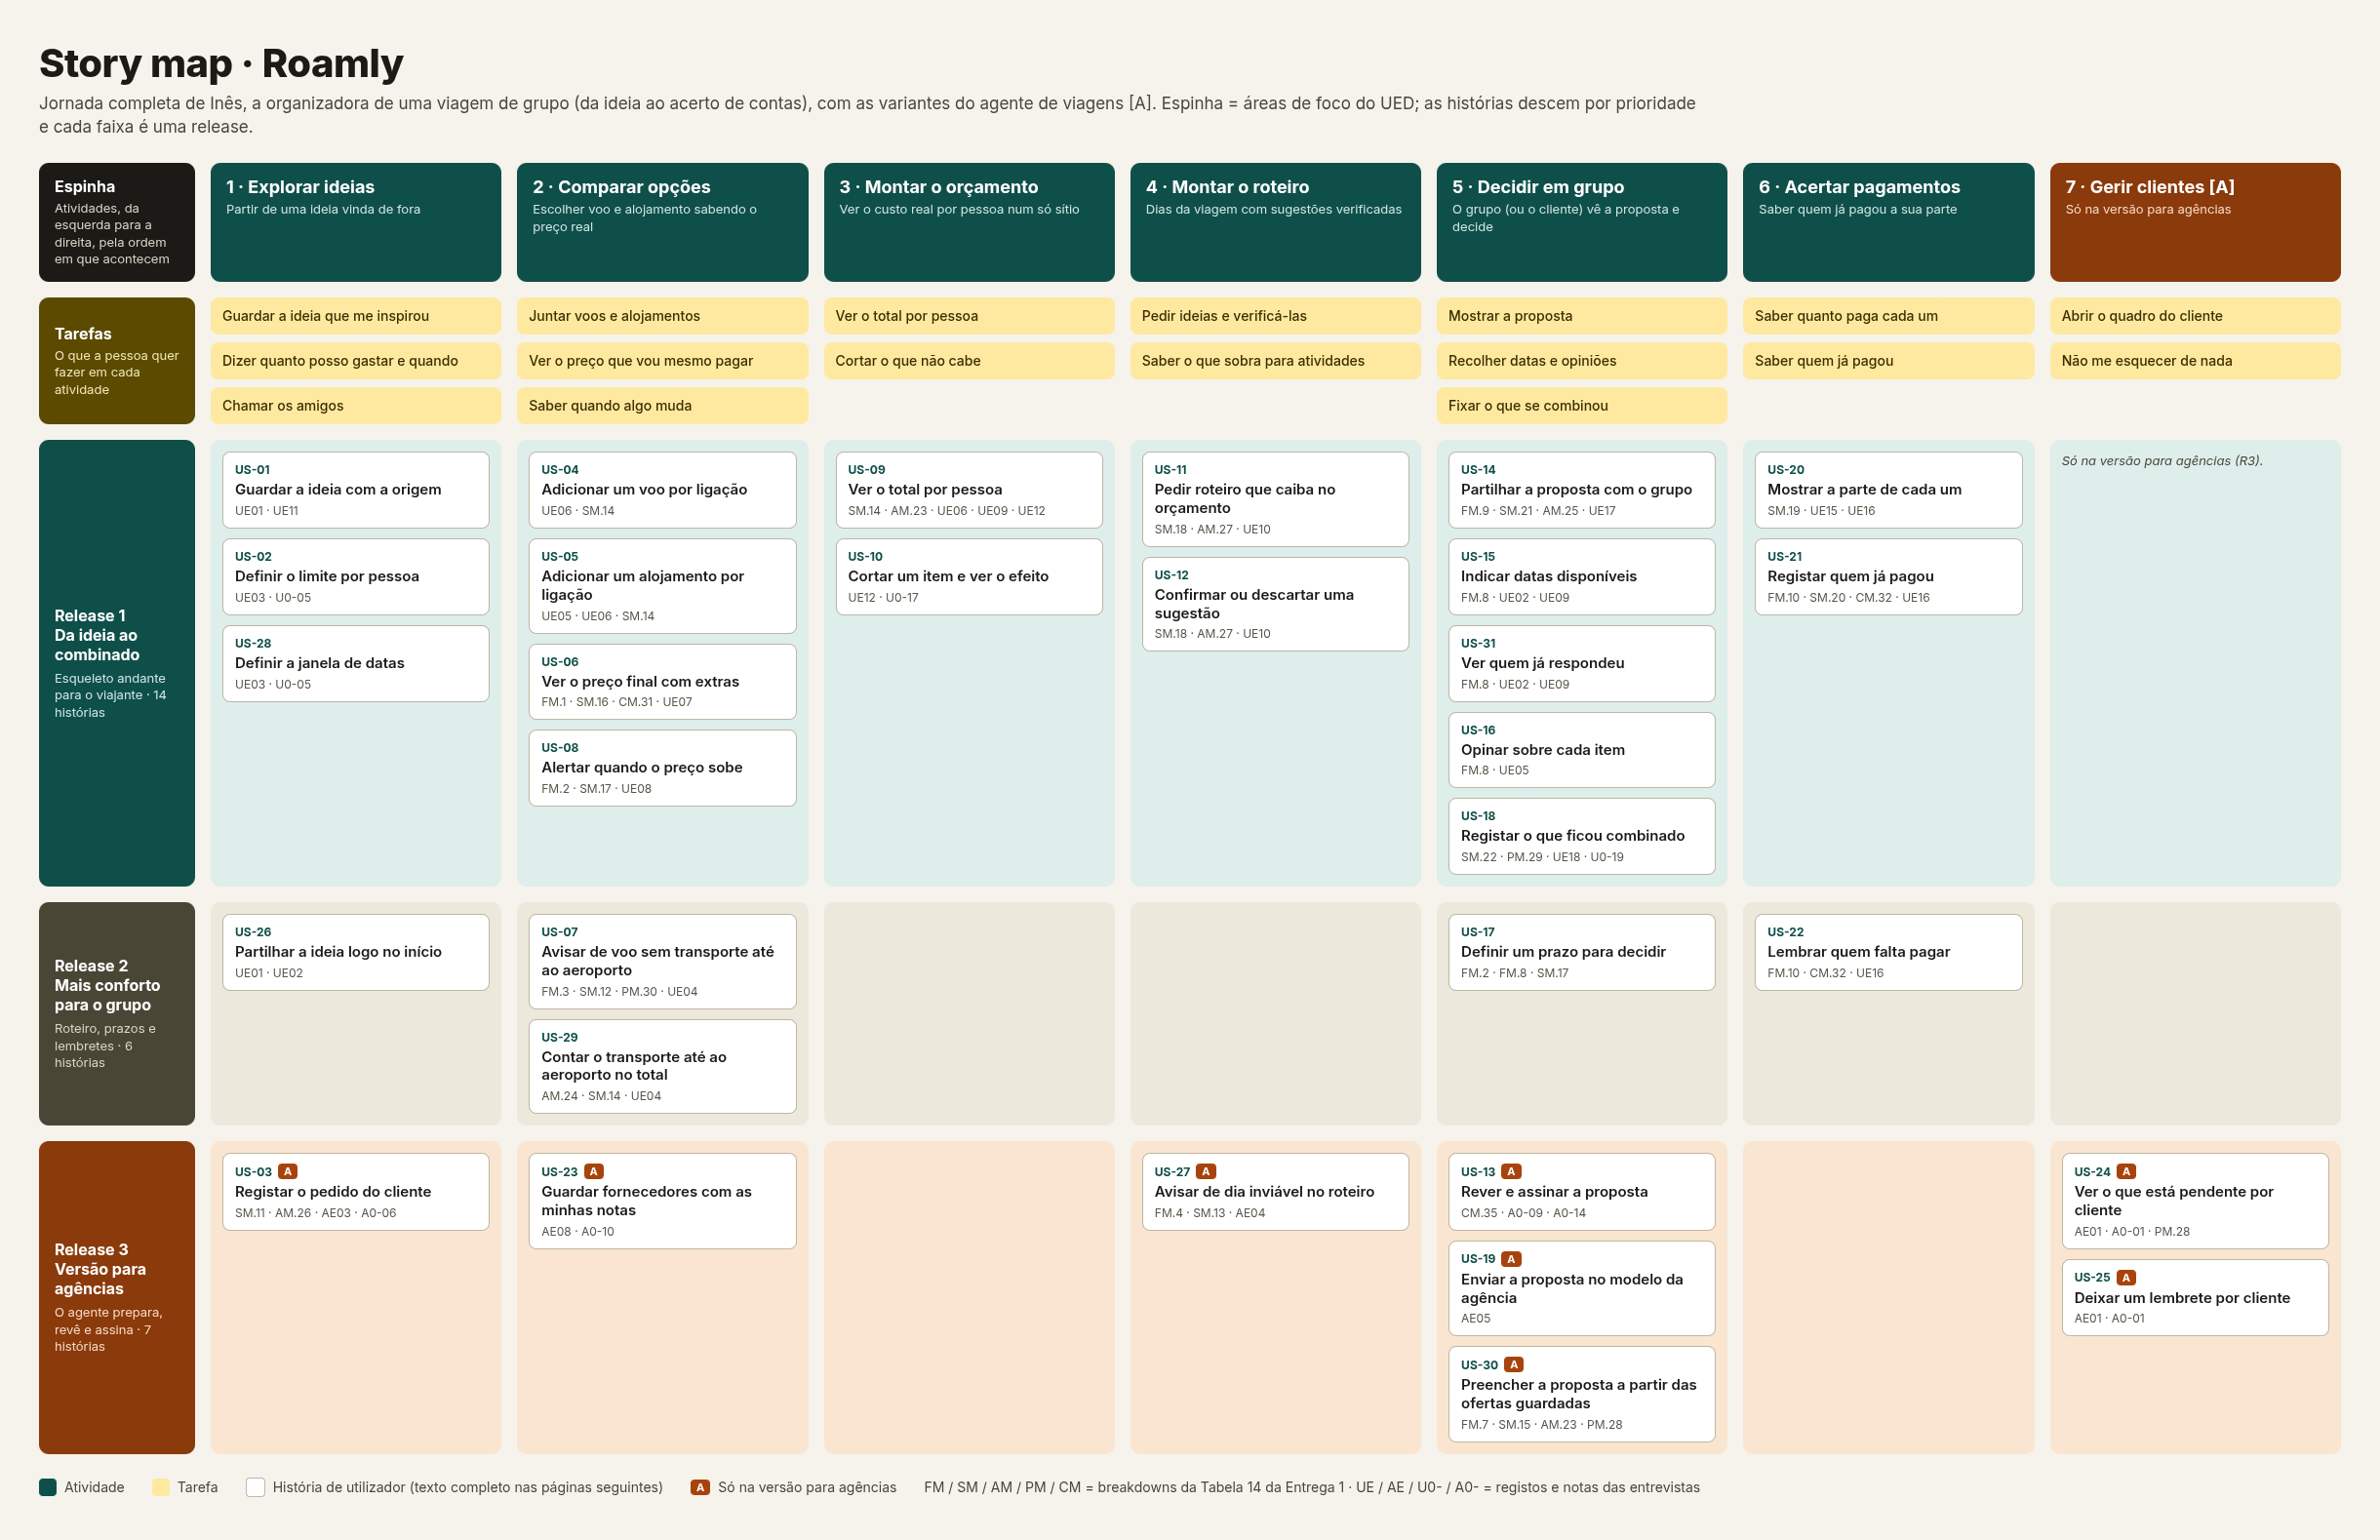
\includegraphics[width=\linewidth,height=0.8\textheight,keepaspectratio]{story_map/story_map.png}
\caption{\textit{Story map} do \projeto.}
\label{fig:storymap}
\end{figure}
\end{landscape}

% Tabela gerada a partir de ../story_map/historias_roamly.md (editar o .md e voltar a gerar)
% Pacotes necessários no preâmbulo: \usepackage{longtable,booktabs,array}
% Cole este bloco no sítio onde quer a tabela (ex.: Secção 2, Story map). [A] = só versão para agências.
{\small
\setlength{\tabcolsep}{4pt}
\begin{longtable}{@{}p{1.5cm}p{5.1cm}p{5.2cm}p{3.6cm}@{}}
\caption{Histórias de utilizador do Roamly, agrupadas por release.}\label{tab:historias}\\
\toprule \textbf{ID} & \textbf{História} & \textbf{Critérios de aceitação} & \textbf{Origem e dependências} \\ \midrule
\endfirsthead
\toprule \textbf{ID} & \textbf{História} & \textbf{Critérios de aceitação} & \textbf{Origem e dependências} \\ \midrule
\endhead
\bottomrule \endfoot
\multicolumn{4}{@{}l}{\textbf{Release 1 — Da ideia ao combinado (esqueleto andante do viajante)}} \\ \midrule
\textbf{US-01}\newline Tam. S & \textbf{Guardar a ideia com a origem.}\newline Como organizadora do grupo, quero colar a ligação de um vídeo ou escrever uma ideia de viagem, para a guardar com a origem à vista em vez de a perder entre abas e capturas de ecrã. & (1) Ao colar uma ligação, a ideia fica guardada com o endereço de origem visível.\newline (2) Se for um vídeo, o Roamly guarda-o sem o interpretar e pede-me o destino em texto. & Origem: UE01, UE11; restrição do UED (a IA só lê texto e ligações) \\ \addlinespace
\textbf{US-02}\newline Tam. S & \textbf{Definir orçamento e datas.}\newline Como organizadora, quero indicar o limite por pessoa e as datas possíveis, para que tudo o que juntar seja comparado com o que o grupo pode gastar. & (1) Guardo um limite por pessoa (ex.: 300 €) e uma janela de datas (ex.: um mês inteiro).\newline (2) O limite fica visível em todas as janelas onde aparecem preços. & Origem: UE03, U0-05; perfil U0 (300 € por pessoa) \\ \addlinespace
\textbf{US-04}\newline Tam. M & \textbf{Adicionar um voo por ligação.}\newline Como organizadora, quero colar a ligação de uma oferta de voo e ver preço, horários e condições lidos automaticamente, para não os copiar à mão para uma folha de cálculo. & (1) Com uma ligação válida, a oferta aparece no Caderno com preço por pessoa e horários, sem eu escrever nada.\newline (2) Se o Roamly não conseguir ler a página, diz-me e deixa-me preencher à mão. & Origem: FM.7, SM.15, PM.28, UE06\newline Depende de: Risco: acesso aos dados dos sites (Secção 2.6) \\ \addlinespace
\textbf{US-05}\newline Tam. M & \textbf{Adicionar um alojamento por ligação.}\newline Como organizadora, quero colar a ligação de um alojamento e ver preço por noite e condições, para o comparar com outros sem abrir um site de cada vez. & (1) A opção aparece com o preço por pessoa e noite e o total para as noites da viagem.\newline (2) Posso abrir o site original em ``Ver no site'' para confirmar a informação. & Origem: FM.7, PM.28, UE05, UE06\newline Depende de: US-04 \\ \addlinespace
\textbf{US-06}\newline Tam. M & \textbf{Ver o preço final com extras.}\newline Como organizadora, quero ver o preço final de um voo já com a bagagem de porão, para não ter surpresas na página de pagamento. & (1) A oferta mostra preço base, extras e ``Preço final''.\newline (2) Se o site não revelar os extras, aparece ``extras por confirmar'' em vez de os omitir. & Origem: FM.1, SM.16, CM.31, UE07 (bagagem +34 €)\newline Depende de: US-04 \\ \addlinespace
\textbf{US-08}\newline Tam. M & \textbf{Alertar quando o preço sobe.}\newline Como organizadora, quero ser avisada quando o preço de uma oferta guardada sobe, para decidir antes de ele subir ainda mais. & (1) O Roamly volta a ler as ligações guardadas e, se o preço subiu, a oferta mostra de quanto.\newline (2) Recebo uma notificação; o Roamly não congela preços nem faz reservas. & Origem: FM.2, SM.17, UE08 (o voo subiu 19 €)\newline Depende de: US-04, US-05 \\ \addlinespace
\textbf{US-09}\newline Tam. S & \textbf{Ver o total por pessoa.}\newline Como organizadora, quero ver num só sítio o total por pessoa das opções escolhidas, para saber se a viagem cabe no limite sem refazer contas à mão. & (1) O total atualiza-se sozinho quando um preço muda.\newline (2) Quando passa o limite, aparece um aviso junto ao total. & Origem: SM.14, AM.23, UE06, UE09, UE12 (303 $\rightarrow$ 322 $\rightarrow$ 294 €) \\ \addlinespace
\textbf{US-10}\newline Tam. S & \textbf{Cortar um item e ver o efeito.}\newline Como organizadora, quero cortar um item e ver logo o novo total, ficando o item riscado e à vista, para mostrar ao grupo o que cortei e porquê. & (1) Ao cortar, o total por pessoa recalcula-se de imediato.\newline (2) O item cortado continua visível, riscado, e posso repô-lo. & Origem: UE12 (mina de sal, 28 €), U0-17\newline Depende de: US-09 \\ \addlinespace
\textbf{US-14}\newline Tam. M & \textbf{Partilhar a proposta com o grupo.}\newline Como organizadora, quero partilhar a proposta numa ligação que os amigos veem sem abrir folhas de cálculo, para deixarem de pedir ``manda print''. & (1) Quem recebe a ligação vê itens, preços e total por pessoa sem abrir mais nada.\newline (2) A proposta partilhada reflete as alterações que eu fizer depois. & Origem: FM.9, SM.21, AM.25, UE17\newline Depende de: US-09 \\ \addlinespace
\textbf{US-15}\newline Tam. S & \textbf{Indicar datas disponíveis.}\newline Como membro do grupo, quero indicar se posso nas datas propostas ou em que outras posso, para o organizador deixar de esperar por respostas soltas. & (1) Escolho a data proposta ou indico a minha.\newline (2) A organizadora vê quem já respondeu e quem falta. & Origem: FM.8, UE02, UE09\newline Depende de: US-14 \\ \addlinespace
\textbf{US-16}\newline Tam. S & \textbf{Opinar sobre cada item.}\newline Como membro do grupo, quero marcar ``Concordo'' ou ``Prefiro outra'' em cada item da proposta, para dizer o que não aceito antes de se reservar. & (1) Cada item (voo, alojamento\ldots{}) mostra a minha resposta e a dos outros.\newline (2) A organizadora vê onde há divergência e só reserva quando todos concordam. & Origem: FM.8, UE05 (``dormitório não'')\newline Depende de: US-14 \\ \addlinespace
\textbf{US-18}\newline Tam. S & \textbf{Registar o que ficou combinado.}\newline Como organizadora, quero registar na própria proposta o que o grupo decidiu, para não ter de o passar a limpo depois de cada conversa. & (1) Escrevo o combinado na proposta e todos os membros o veem.\newline (2) O registo fica junto dos itens a que se refere. & Origem: SM.22, PM.29, UE18, U0-19\newline Depende de: US-14 \\ \addlinespace
\textbf{US-20}\newline Tam. S & \textbf{Mostrar a parte de cada um.}\newline Como organizadora, quero ver quanto cada pessoa paga antes de reservar, para pedir o valor certo e saber quanto vou adiantar. & (1) A parte de cada um é calculada a partir dos itens acordados.\newline (2) Vejo o total que terei de adiantar ao reservar. & Origem: SM.19, UE15, UE16 (98 € a cada amigo)\newline Depende de: US-09 \\ \addlinespace
\textbf{US-21}\newline Tam. S & \textbf{Registar quem já pagou.}\newline Como organizadora, quero marcar que um amigo já me pagou, para saber quem falta sem controlar de cabeça. & (1) Só eu, como organizadora, posso marcar um pagamento como feito.\newline (2) O Roamly não processa pagamentos: apenas regista. & Origem: FM.10, SM.20, CM.32, UE16\newline Depende de: US-20 \\ \addlinespace
\midrule
\multicolumn{4}{@{}l}{\textbf{Release 2 — Mais conforto para o grupo}} \\ \midrule
\textbf{US-26}\newline Tam. S & \textbf{Partilhar a ideia logo no início.}\newline Como organizadora, quero partilhar a ideia guardada com os amigos logo no início, para ver quem alinha antes de gastar tempo a pesquisar. & (1) Posso enviar a ideia guardada aos amigos a partir da janela Pesquisa.\newline (2) Os amigos veem a ideia com a origem e o limite por pessoa. & Origem: UE01, UE02; ligação 1 $\rightarrow$ 5 do UED\newline Depende de: US-01, US-02 \\ \addlinespace
\textbf{US-07}\newline Tam. M & \textbf{Avisar de voo sem transporte até ao aeroporto.}\newline Como organizadora, quero ser avisada quando um voo me obriga a chegar ao aeroporto a uma hora sem transporte, e ver o custo dessa viagem no total, para não escolher um voo que não consigo apanhar. & (1) Ao escolher um voo, aparece um aviso se não há transporte à hora necessária.\newline (2) O custo do transporte até ao aeroporto entra no total por pessoa. & Origem: FM.3, SM.12, AM.24, PM.30, UE04\newline Depende de: US-04, US-09. Risco: precisa de dados de horários de transportes (por confirmar) \\ \addlinespace
\textbf{US-11}\newline Tam. M & \textbf{Pedir um roteiro que caiba no orçamento.}\newline Como organizadora, quero pedir à IA um roteiro que caiba no que sobra do orçamento, para ter ideias de atividades baratas sem passar do limite. & (1) O Roamly mostra quanto sobra por pessoa antes de eu pedir o roteiro.\newline (2) Cada sugestão traz a fonte e o custo. & Origem: SM.18, AM.27, UE10\newline Depende de: US-09 \\ \addlinespace
\textbf{US-12}\newline Tam. S & \textbf{Confirmar ou descartar uma sugestão.}\newline Como organizadora, quero ver cada sugestão no mapa e marcá-la como confirmada ou descartada, para só contar com o que é verdade. & (1) Cada sugestão pode ser aberta no mapa.\newline (2) Fica marcada como confirmada ou descartada e o estado é visível ao grupo. & Origem: SM.18, AM.27, UE10 (confirmou 2, descartou 1)\newline Depende de: US-11 \\ \addlinespace
\textbf{US-17}\newline Tam. S & \textbf{Definir um prazo para decidir.}\newline Como organizadora, quero fixar um prazo para o grupo decidir, para as respostas não ficarem em aberto enquanto o preço sobe. & (1) O prazo aparece a todos os membros na proposta.\newline (2) Se o preço subir antes do prazo, o grupo é avisado. & Origem: FM.2, FM.8, SM.17\newline Depende de: US-08, US-14 \\ \addlinespace
\textbf{US-22}\newline Tam. S & \textbf{Lembrar quem falta pagar.}\newline Como organizadora, quero que o Roamly lembre quem ainda não me pagou, para não ter de cobrar eu a cada amigo. & (1) Quem não está marcado como pago recebe um lembrete.\newline (2) Posso decidir quando o lembrete é enviado. & Origem: FM.10, CM.32, UE16 (``só no fim do mês'')\newline Depende de: US-21 \\ \addlinespace
\midrule
\multicolumn{4}{@{}l}{\textbf{Release 3 — Versão para agências}} \\ \midrule
\textbf{US-03} [A]\newline Tam. S & \textbf{Registar o pedido do cliente.}\newline Como agente de viagens, quero registar o roteiro que o cliente traz, com o orçamento, as datas flexíveis e ``o que não abdicam'', para não perder o que o roteiro não diz. & (1) O pedido guarda o roteiro (ligação ou texto) e os três campos.\newline (2) Se faltar algum dos três, o pedido assinala-o antes de eu montar a proposta. & Origem: SM.11, AM.26, AE03, A0-06\newline Depende de: US-24 \\ \addlinespace
\textbf{US-23} [A]\newline Tam. S & \textbf{Guardar fornecedores com as minhas notas.}\newline Como agente de viagens, quero guardar fornecedores que não estão online, com as minhas notas, para os ter à mão ao montar propostas e não só no caderno. & (1) Guardo um fornecedor com notas (ex.: ``pedir quarto nos pisos de cima'').\newline (2) As opções guardadas aparecem junto das outras no Caderno. & Origem: AE08, A0-10; persona Rui \\ \addlinespace
\textbf{US-27} [A]\newline Tam. M & \textbf{Avisar de dia inviável no roteiro.}\newline Como agente de viagens, quero ser avisado quando um dia do roteiro que o cliente traz não é viável (deslocações longas, sítios fechados), para não montar uma proposta que não funciona. & (1) O aviso diz qual é o dia e a razão (ex.: duas cidades a 6 h de comboio).\newline (2) Posso ignorar o aviso e manter o dia. & Origem: FM.4, SM.13, AE04\newline Depende de: US-03 \\ \addlinespace
\textbf{US-13} [A]\newline Tam. M & \textbf{Rever e assinar a proposta.}\newline Como agente de viagens, quero rever e assinar a proposta preparada pela IA antes de o cliente a ver, para nada chegar ao cliente sem a minha validação. & (1) O cliente não vê a proposta enquanto eu não a assinar.\newline (2) Posso alterar qualquer item antes de assinar. & Origem: CM.35, A0-09, A0-14; Secção 6.2 (referida como US-13)\newline Depende de: Questão em aberto: como sabe o cliente que a proposta foi revista por uma pessoa? \\ \addlinespace
\textbf{US-19} [A]\newline Tam. M & \textbf{Enviar a proposta com o logótipo da agência.}\newline Como agente de viagens, quero enviar ao cliente a proposta com o logótipo da agência e os preços atualizados, sem copiar dados do portal, para responder depressa. & (1) A proposta sai no modelo da agência, com o logótipo.\newline (2) Os dados vêm das ofertas guardadas, não de cópia manual. & Origem: FM.7, SM.15, AE05, FM.6 (taxa de serviço)\newline Depende de: US-13 \\ \addlinespace
\textbf{US-24} [A]\newline Tam. S & \textbf{Abrir um quadro por cliente.}\newline Como agente de viagens, quero abrir ou criar um quadro por cliente e ver o que está pendente, para trabalhar num só sítio em vez de várias aplicações. & (1) Posso criar um quadro para um cliente novo.\newline (2) Cada quadro mostra os pedidos novos e as propostas por enviar. & Origem: AE01, A0-01, PM.28 \\ \addlinespace
\textbf{US-25} [A]\newline Tam. S & \textbf{Deixar um lembrete no quadro.}\newline Como agente de viagens, quero deixar um lembrete no quadro do cliente, para deixar de depender do papel autocolante no monitor. & (1) O lembrete (ex.: ``ligar ao cliente X'') fica no quadro desse cliente.\newline (2) Os lembretes pendentes aparecem junto do que está por fazer. & Origem: AE01, A0-01\newline Depende de: US-24 \\ \addlinespace
\midrule
\end{longtable}
}

